\documentclass{beamer}
\usepackage[orientation=portrait,size=a0,scale=1.2,debug]{beamerposter}
\mode<presentation>{\usetheme{ZH}}
\usepackage[none]{hyphenat}
\usepackage{mathspec}
\setallmainfonts{Archivo Narrow}
\setsansfont[BoldFont={Roboto Condensed Bold}]{Roboto Condensed}
\setmonofont[BoldFont={Inconsolata}]{Inconsolata}
\newfontfamily\titlefont[BoldFont={Archivo Narrow}]{Archivo Narrow}
\usepackage{hyperref} %enable hyperlink for urls
\usepackage{ragged2e}
\let\raggedright=\RaggedRight
\usepackage[font=small,margin=50pt,labelfont=bf,justification=justified, compatibility=false]{caption}

\usepackage{array,booktabs,tabularx}

\newcolumntype{Z}{>{\centering\arraybackslash}X} % centered tabularx columns
%\sisetup{per=frac,fraction=sfrac}

\title{\titlefont{Crystal structure prediction for next-generation battery anodes}}
\author{\titlefont{\underline{Matthew L. Evans}$^{1,\,\dagger}$, Kent J. Griffith$^2$, Andrew J. Morris$^1$}}
\institute{\titlefont{$^1$ TCM Group, Cavendish Laboratory, University of Cambridge\\[.2in]$^2$ Department of Chemistry, University of Cambridge}}

% edit this depending on how tall your header is. We should make this scaling automatic :-/
\newlength{\columnheight}
\setlength{\columnheight}{104cm}

\begin{document}
\begin{frame}
    \begin{columns}
        \begin{column}{.01\textwidth}
        \end{column}
	\begin{column}{.57\textwidth}
		\begin{beamercolorbox}[center]{postercolumn}
			\begin{minipage}{.98\textwidth}  % tweaks the width, makes a new \textwidth
				\parbox[t][\columnheight]{\textwidth}{ % must be some better way to set the the height, width and textwidth simultaneously
            \begin{myabstract}{Abstract}
                In this work, we perform \textbf{high-throughput crystal structure prediction} on materials that have great promise as conversion anodes for next-generation Li-, Na- and K-ion batteries, namely metal phosphide alloys. Using \emph{ab initio} random structure searching \cite{Pickard2011} and related methods, previous work on phosphorus anodes \cite{Mayo2016} is extended in an attempt to find \textbf{sustainable materials} with \textbf{manageable volume expansion} during charging.
            \end{myabstract}
            \begin{columns}
	\begin{column}{.48\textwidth}
		\begin{beamercolorbox}[left]{postercolumn}
        \begin{minipage}{\textwidth}  % tweaks the width, makes a new \textwidth
				\parbox[t][\columnheight]{\textwidth}{ % must be some better way to set the the height, width and textwidth simultaneously
            \begin{myblock}{\titlefont{Motivation}}
                  In order to displace fossil fuels in the global energy infrastructure, sustainable, high-capacity energy storage solutions are urgently required. Lithium-ion batteries have already revolutionised the world, bringing about the advent of portable electronics --- how can we extend this technology to grid applications?

            Graphite anodes for Li-ion batteries have theoretical gravimetric capacity of 372 mAh/g (LiC$_6$). These anodes are limited in rate capability by the sluggishness of the intercalation process --- charging too rapidly leads to Li plating and dangerous shorting of the cell. As an alternative, materials that alloy with Li, e.g. Si or P, can be used to greatly increase capacity by an order of magnitude (2597 mAh/g for Li$_3$P). This increased capacity comes at the expense of extreme volume expansion, reducing cyclability and safety.

                  \begin{figure}[h]
              \centering
              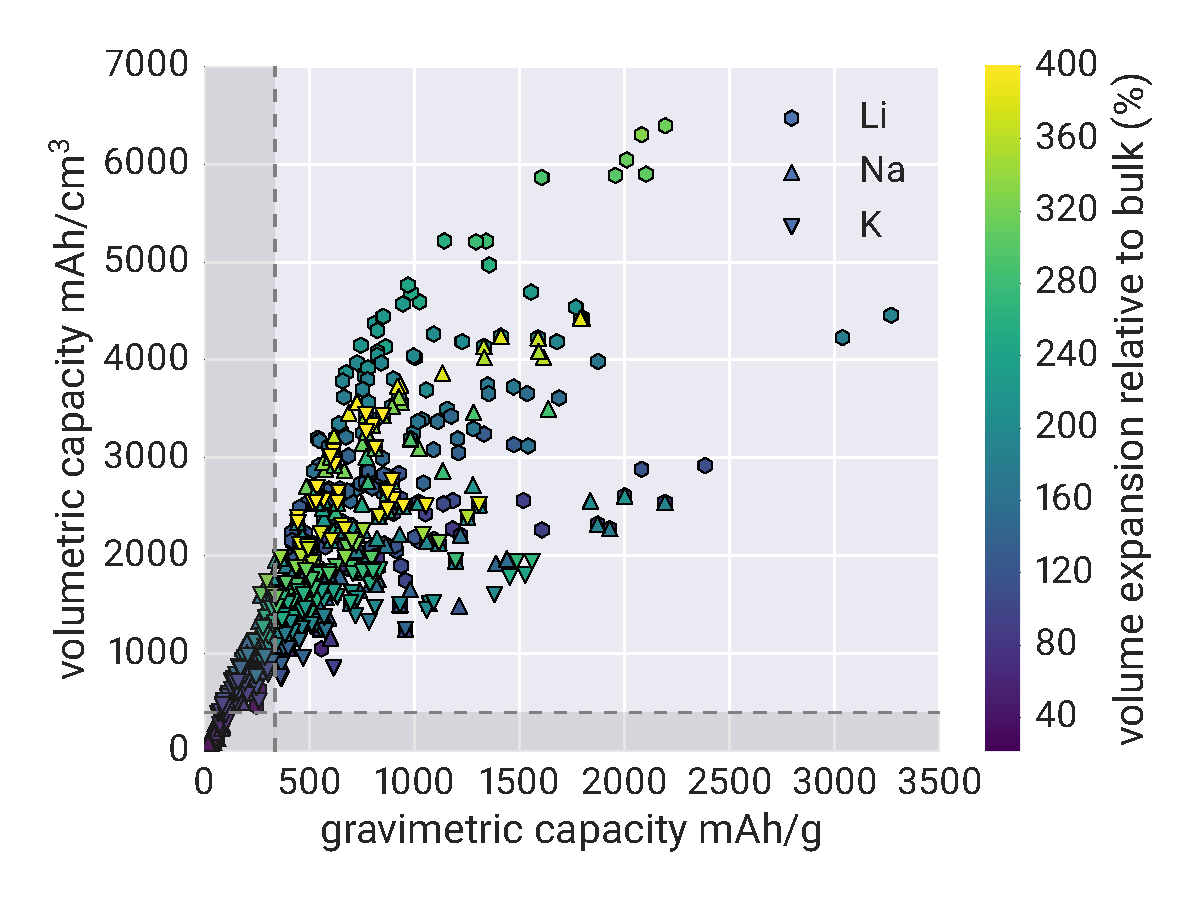
\includegraphics[width=\textwidth]{img/anodes.pdf}
              %\captionsetup{width=0.9\textwidth}
              \caption{Theoretical capacities of ternary conversion anodes for Li-, Na- and K-ion batteries, using known phases from the OQMD \cite{Kirklin2015}.}
            \end{figure}
Conversion anodes are a middle ground: these binary compounds can exhibit intercalation, alloying and displacement reactions upon cycling. The elements A and B can be tuned such that one forms high-capacity alloys (e.g. P) and the other acts as an inactive (or less active) buffer matrix that ameliorates volume expansion.

					\end{myblock}
					\begin{myblock}{Phosphide conversion anodes}
              An idealised conversion reaction for an X$_x$P$_y$ binary can be described by:
          \[ \text{X}_x \text{P}_y + z\,\text{Li}^+ \to n\,\text{Li}_\delta\text{X}_{x'} + y\,\text{Li}_3\text{P}.\]

          Conversion anodes store Li by converting the original anode material into an Li-rich phase, plus a displaced phase (which may itself contain Li). By mapping out the ternary configuration space, the stable reaction pathways can be enumerated and ranked by thermodynamic and kinetic preferability. Due to the size of the materials space, we focus on sustainable, low-cost potential anode materials, \{Li, Na, K\}-\{Ti, Cu, Zn, Al, Sn\}-P, most recently X-Sn-P.
          \begin{figure}[h]
              \centering
              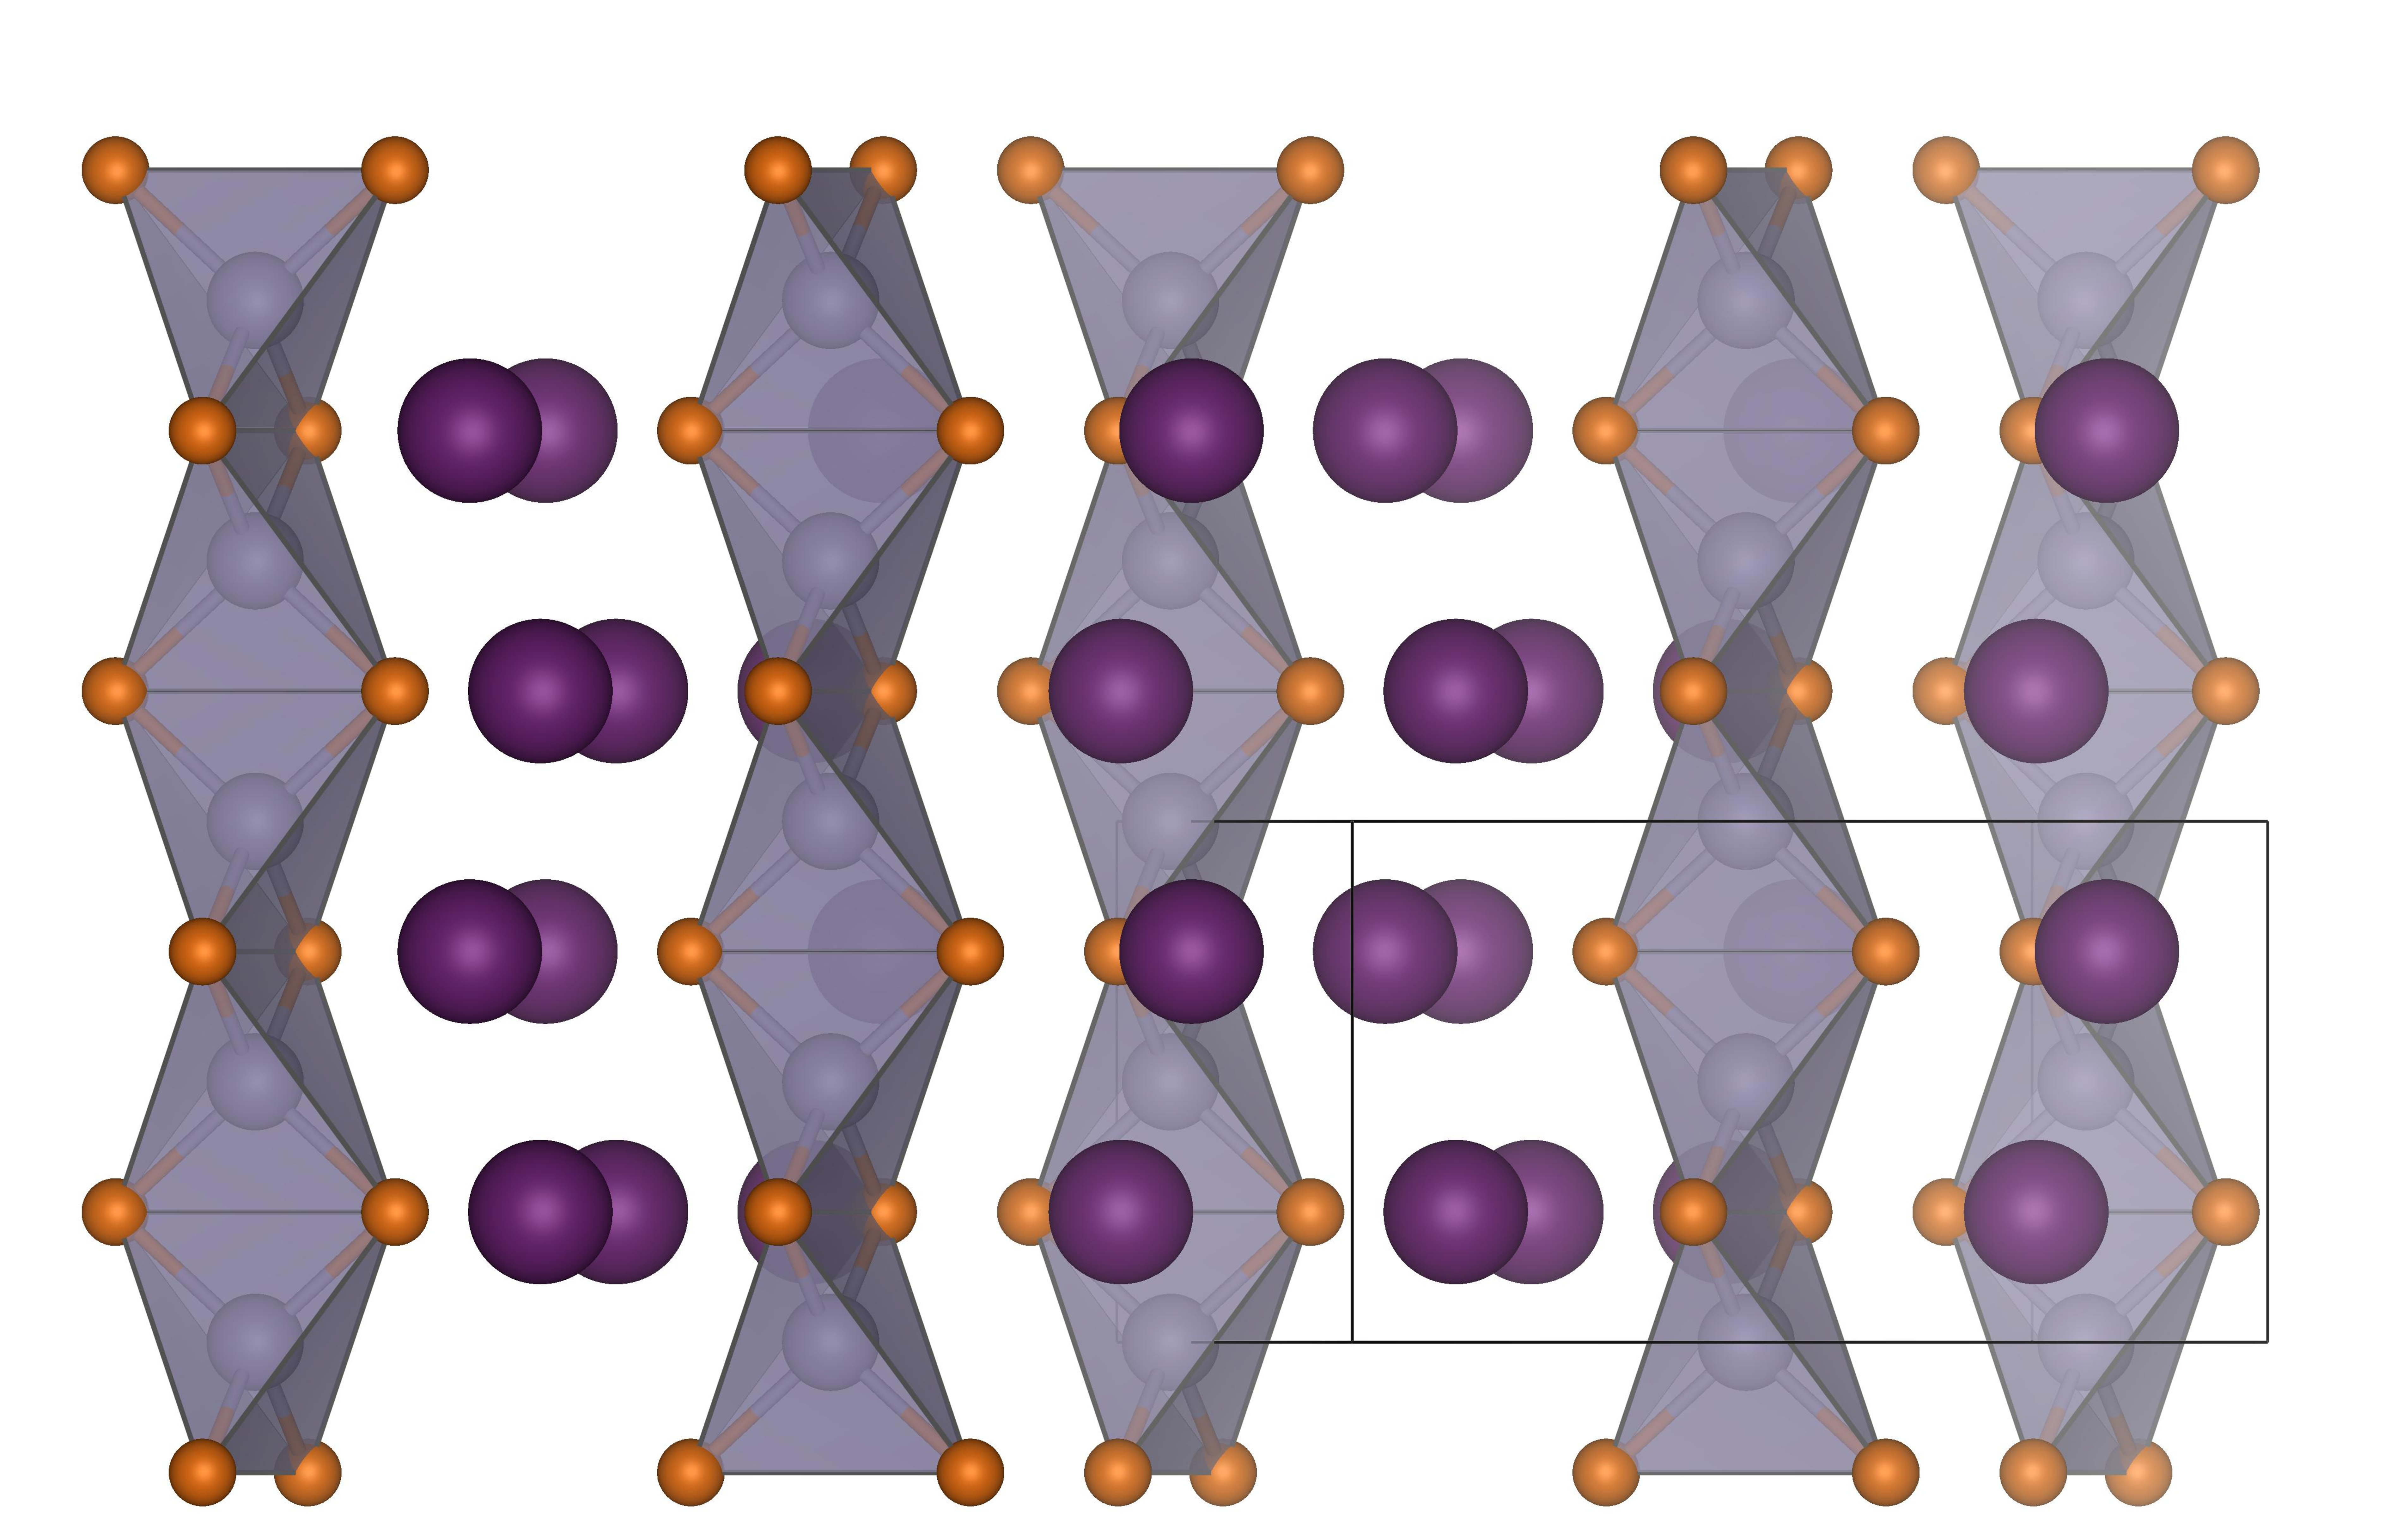
\includegraphics[width=0.7\textwidth]{img/K2P2Sn.pdf}
        \end{figure}
              \vskip-.5cm
    \end{myblock}
		}\end{minipage}\end{beamercolorbox}
	\end{column}
    % no idea why this is needed for proper spacing
  \begin{column}{.00\textwidth}
    \end{column}
  \begin{column}{.48\textwidth}
		\begin{beamercolorbox}[right]{postercolumn}
			\begin{minipage}{\textwidth} % tweaks the width, makes a new \textwidth
				\parbox[t][\columnheight]{\textwidth}{ % must be some better way to set the the height, width and textwidth simultaneously
					\begin{myblock}{Crystal structure prediction}
              Broadly, crystal structure prediction is the act of searching for the lowest energy configurations of atoms under different conditions. When modelling batteries, we sample various compositions as if the system were connected to an infinite reservoir of the active ion.
              
              The primary method used here to perform  an unbiased sampling across various compositions is \emph{ab initio} random structure searching (AIRSS) \cite{Pickard2011}. By randomly generating many structures with \emph{sensible} symmetries and connectivities and relaxing them with forces from rough density-functional theory (DFT) calculations, the energy landscape can be efficiently mapped. Computing the convex hull of formation energies against elemental (or otherwise) chemical potentials yields the zero-temperature phase diagram of the system.
            \begin{figure}
                \centering
              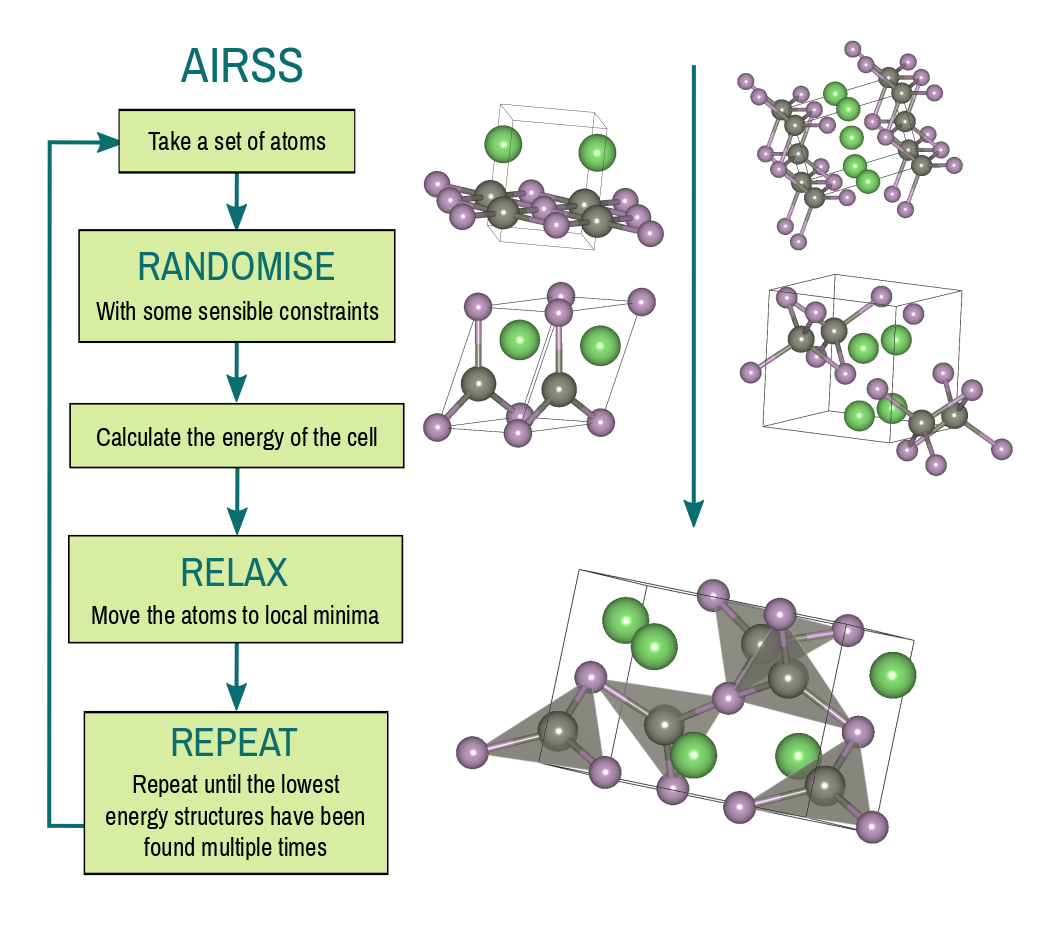
\includegraphics[width=\textwidth]{img/airss.png}
          \end{figure}
              
              With sufficient sampling, AIRSS will find the global minima at each stoichiometry, however, when the search space is very large, this may require hundreds of thousands of calculations. Exploiting experimental and theoretical databases by swapping atomic types from known crystal structures will often yield undiscovered structures; this data mining approach can be thought of as an interpolation of chemical trends.
                \vspace{0.2in}
              \begin{figure}
                \centering
              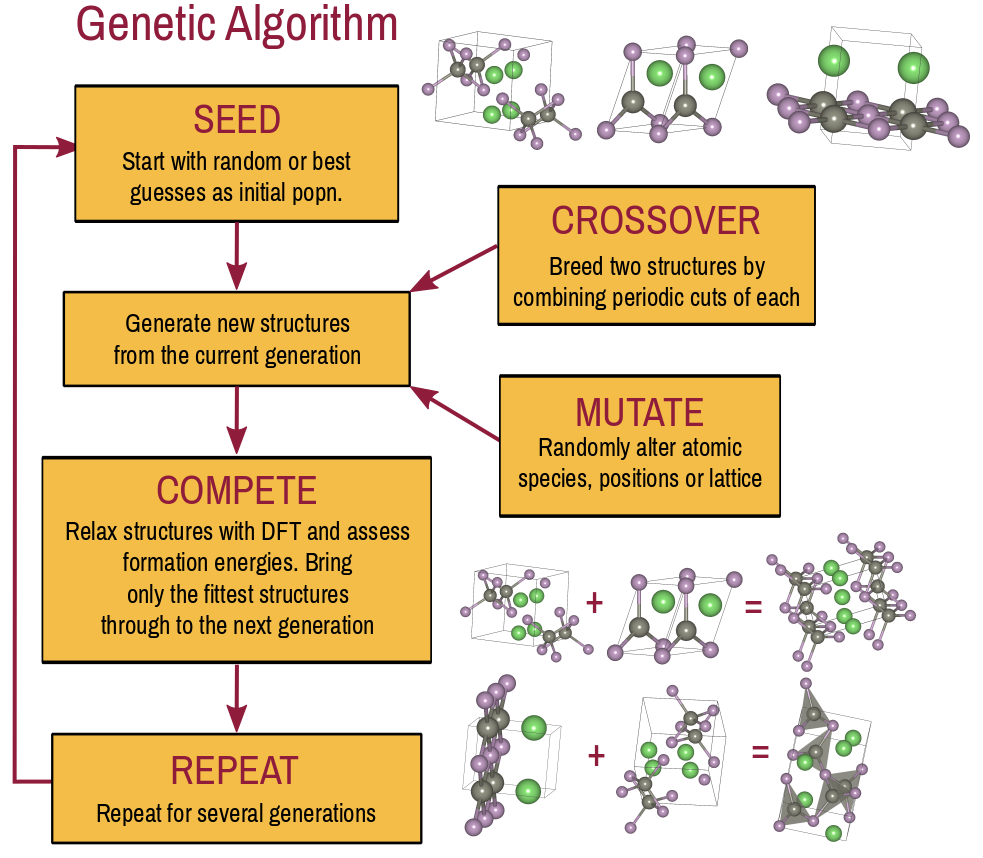
\includegraphics[width=\textwidth]{img/ga.png}
          \end{figure}

Even with very few trials, AIRSS will often find the correct local structure at a given stoichiometry --- we seed a genetic algorithm with interim AIRSS results to exploit this fact. Starting from an initial population, structures are randomly mutated and combined, relaxed and then ranked by ``fitness'' (formation energy) to form the next generation. This is repeated for many generations until no new structures are found (stagnation).

					\end{myblock}\vfill
		}\end{minipage}\end{beamercolorbox}
	\end{column}
  \end{columns}
		}\end{minipage}\end{beamercolorbox}
  \end{column}
    
	\begin{column}{.37\textwidth}
		\begin{beamercolorbox}[center]{postercolumn}
			\begin{minipage}{.98\textwidth} % tweaks the width, makes a new \textwidth
				\parbox[t][\columnheight]{\textwidth}{ % must be some better way to set the the height, width and textwidth simultaneously
            \begin{myblock}{Results}


                An example of proof-of-concept results for the Li-Zn-P system are shown below, the result of around 10,000 DFT relaxations. We have studied the P-Sn system for Li, Na and K in much more detail (100k structures per phase diagram).

            \begin{figure}
                \centering
              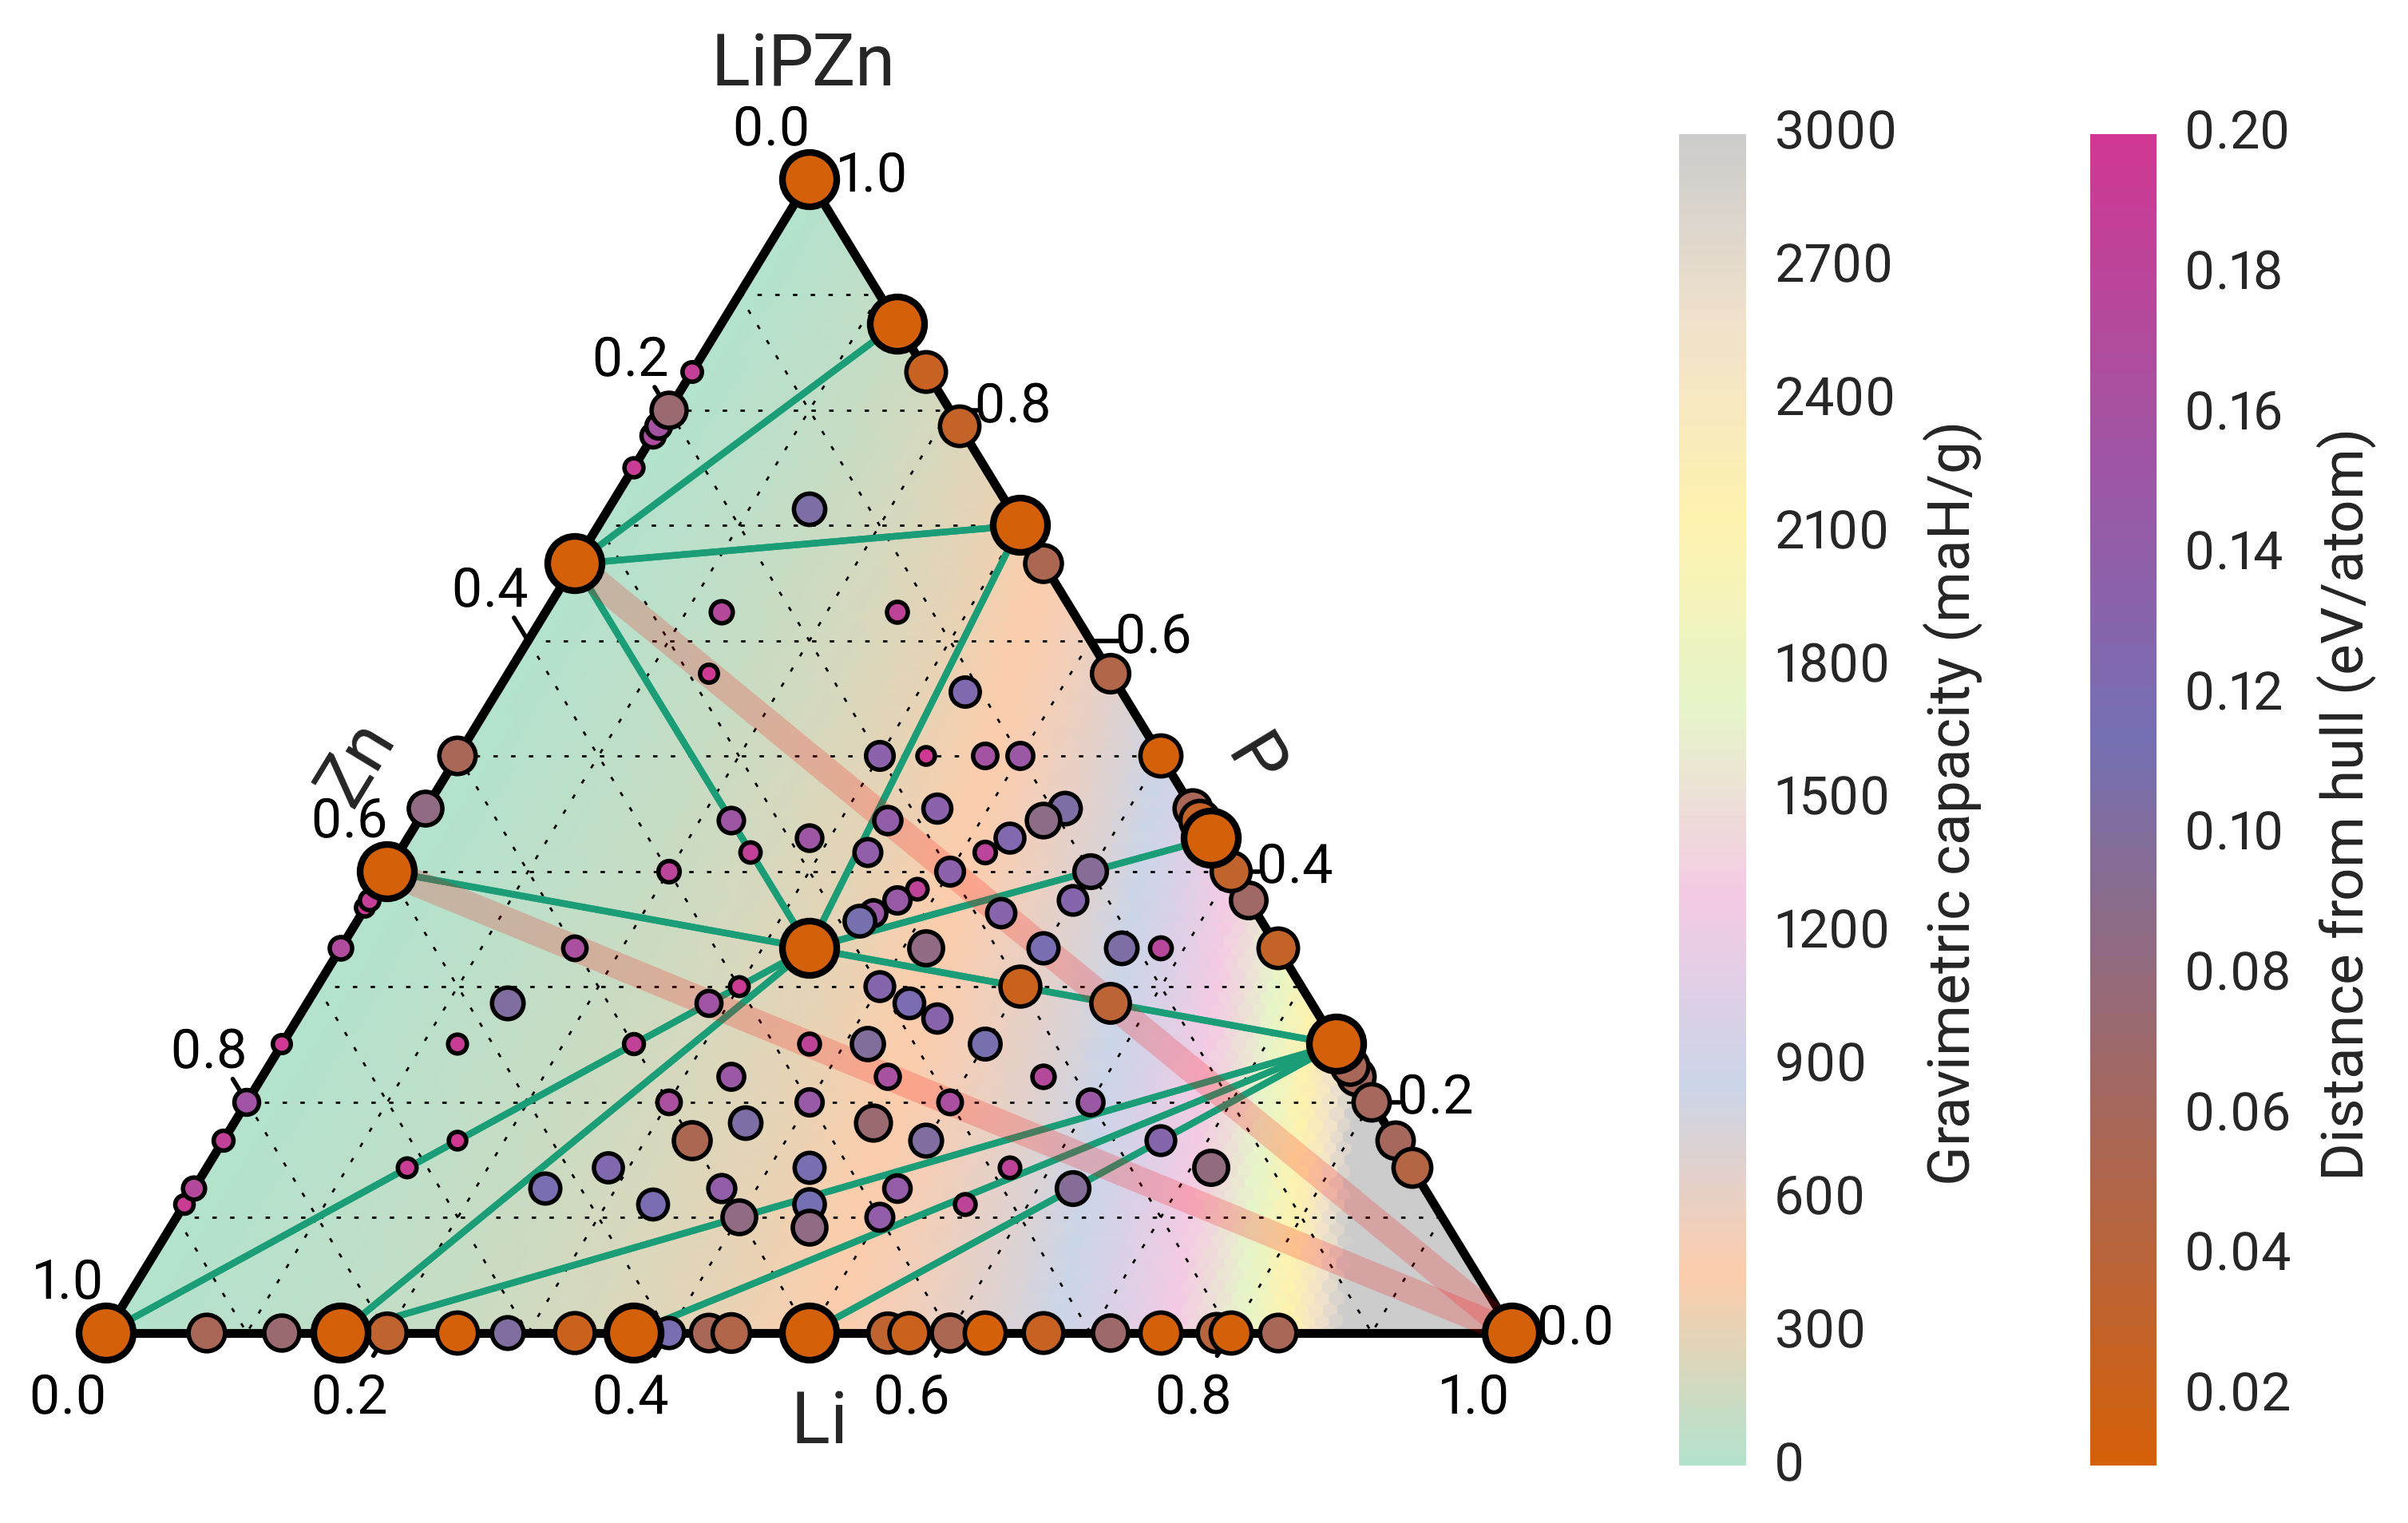
\includegraphics[width=\textwidth]{img/LiPZn.png}
              %\captionsetup{margin=20pt, width=0.9\textwidth}
              \caption{Ternary phase diagram of the Li-P-Zn system, with points coloured by degree of metastability, and space coloured by gravimetric capacity at that composition. Red lines show the pathways from delithiated phases to pure Li.}
            \end{figure}

            \begin{itemize}
                \item The lowest energy structures from the searching stage are re-relaxed at higher level of accuracy, in order to compute voltage curves to compare with experiment.
                \item These calculations predict maximum gravimetric capacities of the two known Zn-P alloys as 1473 mAh/g and 934 mAh/g for ZnP$_2$ and Zn$_3$P$_2$ respectively, with manageable volume expansions of 147\% and 122\%.
                \item Each phase exhibits an insertion voltage of around 1 V, suitably high to prevent lithium dendrite formation.
            \end{itemize}
            \begin{figure}
                \centering
              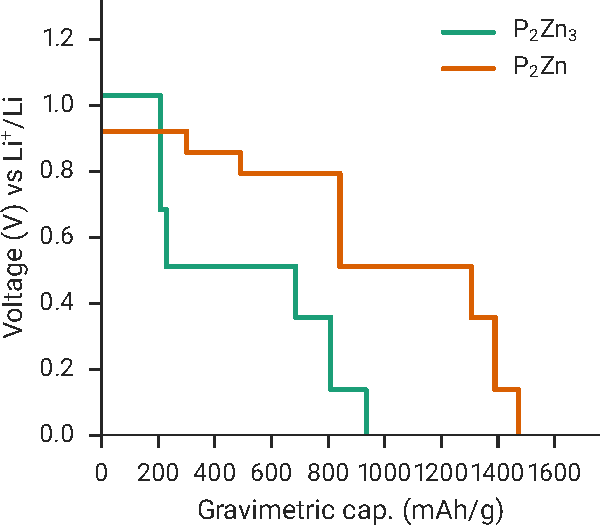
\includegraphics[width=0.6\textwidth]{img/LiPZn_voltage}
              \caption{Predicted 0 K charge/discharge profiles of Zn\textsubscript{3}P\textsubscript{2} and ZnP\textsubscript{2}.}
            \end{figure}

            \begin{itemize}
                \item Several novel metastable phases are predicted (e.g Li$_4$P$_2$Zn, Li$_5$P$_3$Zn$_2$). Knowledge of these metastable phases allows us to calculate the charge/discharge profiles for each of these pathways for comparison with experiment.
            \end{itemize}

          \end{myblock}
          \begin{myblock}{Summary \& Outlook}
              \begin{itemize}
                  \item We are performing computational crystal structure prediction across a region of materials space with great promise for sustainable, high-capacity anodes for Li-, Na- and K-ion batteries.
                  \item Once each phase diagram is complete, electrochemical and spectroscopic properties can be computed and used in conjunction with experiment to improve our understanding of the mechanisms of electrode cycling.
                  \item Metastable phases can be included into our model to investigate the effects of finite-temperature and crystalline disorder on our predictions.
                \end{itemize}
            \end{myblock}
					\begin{myblock}{References}
						\footnotesize
            \bibliographystyle{unsrt}
						\bibliography{references}
					\end{myblock}\vfill
		}\end{minipage}\end{beamercolorbox}
	\end{column}
  \begin{column}{0.01\textwidth}
    \end{column}
\end{columns}
\end{frame}
\end{document}
